\section{INTRODUCTION}
It is known that Wi-Fi access points are vulnerable to remote access of unauthorized users. This research project tries to check the possibility of using location based authentication mechanism for Wi-Fi access point rather than using WPA/ WPA-2 authentication protocols. Location of the user will be measured with respect to user experienced Wi-Fi access point signal strength.

\paragraph{}
This chapter describes techniques related to the research methodology, design of the proposed system and steps that had been carried out to develop the proposed approach. 

\section{BACKGROUND}
\subsection{INVERSE SQUARE LAW}
It can be proven that Wi-Fi access point's signal strength is inversely proportional to the square of distance between device and access point which denotes by the \textbf {Inverse square law} \ref{eq:1}.

\begin{figure}[h]	
	\centering
	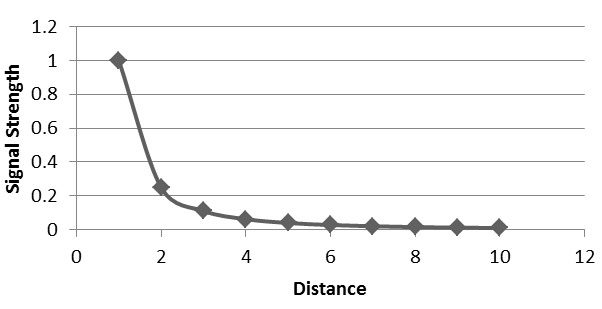
\includegraphics[width=\textwidth]{inverse_square_law.png}
	\caption{Inverse square Law}
\end{figure}

\begin{equation}\boldmath\label{eq:1}
	\beta=\frac{1}{d^2}
\end{equation}\newline


Where:\\
\hspace*{3em}
\begin{tabular}{rl}
	$\beta$:&   received signal strength. \\
	$d$:&  distance between device and access point. \\
\end{tabular}\newline

\paragraph{}
As per the Inverse square law \ref{eq:1}, the received signal strength depends on the distance between user and access point, which means when user goes away from the access point, it results the low received signal strength and wise verse.

\paragraph{}
If the access point is fixed somewhere, it is possible to notice the different level of signal strengths from Wi-Fi access point as per distance.
By using access point's received signal strength, it is possible to identify location uniquely. There are techniques which can be used to identify locations uniquely by using the received signal strength of the Wi-Fi access point.


\subsection{FREE SPACE PATH LOSS}
Since there is a close relationship between received signal strength of the Wi-Fi access point and the distance, distance can be calculated by using following mathematical expression \ref{eq:2}.\newline

	\begin{equation}\boldmath\label{eq:2}
		FSPL(db) = 20\log{10}(d)+20\log{10}(f)+20\log{10}(\frac{4\pi}{c})
	\end{equation}\newline
	
	Where:\\
	\hspace*{3em}
	\begin{tabular}{rl}
		$FSPL(db)$:&   free-space path loss in decibels(received signal strength). \\
		$d$:&  distance between device and access point. \\
		$f$:&  frequency of the access point. \\
		$c$:&  velocity of light in vacuum. \\
	\end{tabular}\newline

\paragraph{}
Free Space Path Loss(FSPL) is defined as \textbf{"The loss between two isotropic radiators in free space, expressed as a power ratio"} \cite{FSPL}
The equation is valid only in an open space(without any obstacles) and here, it cannot be applied directly because the experiment is going to carry out in an environment, which has physical obstacles and also electromagnetic reflection and diffraction.\newline

%\paragraph{}
%The following techniques are used to carry out the project.
\subsection{LOCATION FINGERPRINT TECHNIQUE}

Location fingerprinting technique, which is used to identify each point of the location uniquely according to the RSSI level. In order to fingerprint each point of the desired location, the Wi-Fi access point should be fixed somewhere. Each point's RSSI level changes according to the distance from access point, which makes unique location fingerprint according to the RSSI level. This makes a new location map with respect to RSSI level. Likewise any other maps like Google map uses the combination of latitude and longitude to identify each location uniquely, here the RSSI level will be used to identify the location.

\paragraph{}
This technique requires combination of a radio frequency and map geographical coordinates. The location will be treated as 2-dimension(2D) cartesian plain together with RSSI values.

\paragraph{}
The location fingerprint technique consists of two main phases.
	\begin{enumerate}
		\item Offline training phase
		\subitem Offline survey phase is most important and most critical in this technique. This is a survey of IEEE 802.11 a/b/g/n Wi-Fi signal strength of desired survey area(location which is going to be fingerprint). 
		\paragraph{}
		First, the survey area should be divided into the size of ($1m\times1m = 1m^2$). It is free to decide the area size as per the requirement. But for more accurate survey, more readings are required.
			\begin{figure*}[h]	
				\centering
				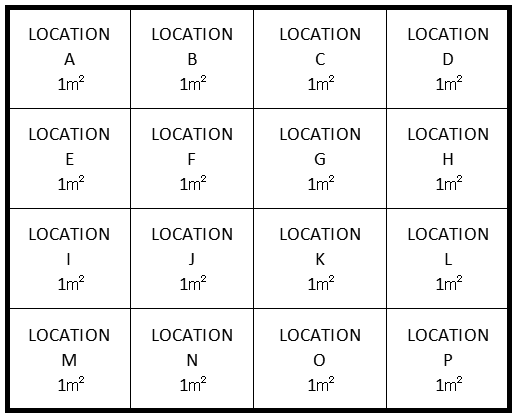
\includegraphics[width=0.5\textwidth]{fp.png}
				\caption{Wi-Fi fingerprinting within area}
			\end{figure*}
		
		Then, the RSSI level of each place should be taken carefully. For more accurate values,the readings(RSSI value) of each location should be taken at least ten(10) times. These readings are stored in a training database which will be used for future assessments of the location.
		
		After this exercise is completed, it is possible to have an average RSSI value of each place. It results a set of data about RSSI level with respect to each location. According to this results, each place can be uniquely identified by using RSSI value for given access point. This is called the location fingerprinting according to the Wi-Fi signal strength.
		
		\begin{description}
			\item NOTE: 
			\subitem Since Wi-Fi signal strength relates with the distance as per the equation \ref{eq:1}, the Access point should be fixed permanently. If the Access point location is changed or Access point hardware is changed, the process should be done from the beginning and training database should be populated with fresh RSSI information. 
		\end{description}
		
		\item Online positioning phase
		\subitem This is where the previous training database is in use. Pointing the user's location by comparing real time data with the information that had been captured in previous phase (known as training database). If offline training phase was completed successfully, online positioning phase can be done quiet easily with more accurate results.
		
		\subitem 
		Wi-Fi signal information (RSSI values) should be captured at real time and it has to be passed to  the place where the position is going to be calculated(server). This server uses the training database and compares the provided Wi-Fi signal strengths with training database data. From that, it can be detected the user's location with respect to Wi-Fi signal strength.
	\end{enumerate}


\subsection{TRILATERATION TECHNIQUE}
The process of calculating the position of the object by using a mathematical way is called "Trilateration".\cite{trilateration} Suppose there are three signal generators A,B,C located in a cartessian plain and each signal generator can fully cover the whole area by itself. 

		\begin{figure*}[h]	
			\centering
			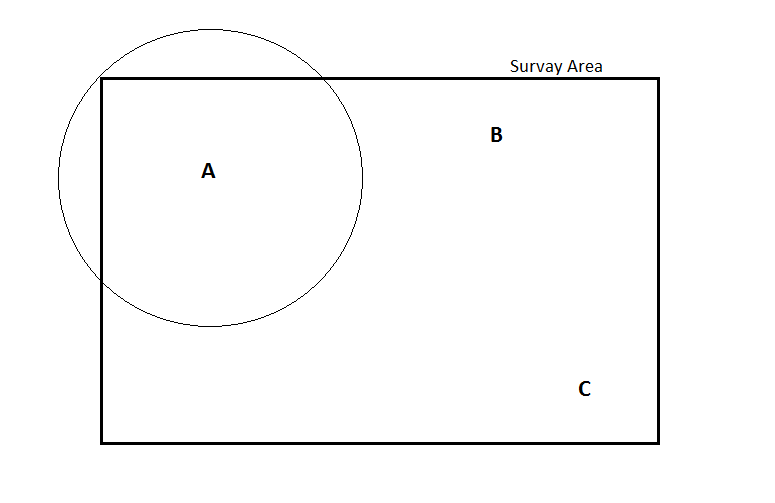
\includegraphics[width=0.8\textwidth]{tri_1.png}
			\caption{Trilateration - Signal Generator A's coverage }
		\end{figure*}

Signal generator(A) generates a signal with specific time and distance and broadcasts that particular signal over air. Even though this signal hits the receiver by any angle, it provides the distance. So this distance forms a circle with a radius of itself. Which means the receiver's location could be anywhere on this circle. Likewise the second signal generator(B)'s signal is also received by the receiver.

\begin{figure*}[h]	
	\centering
	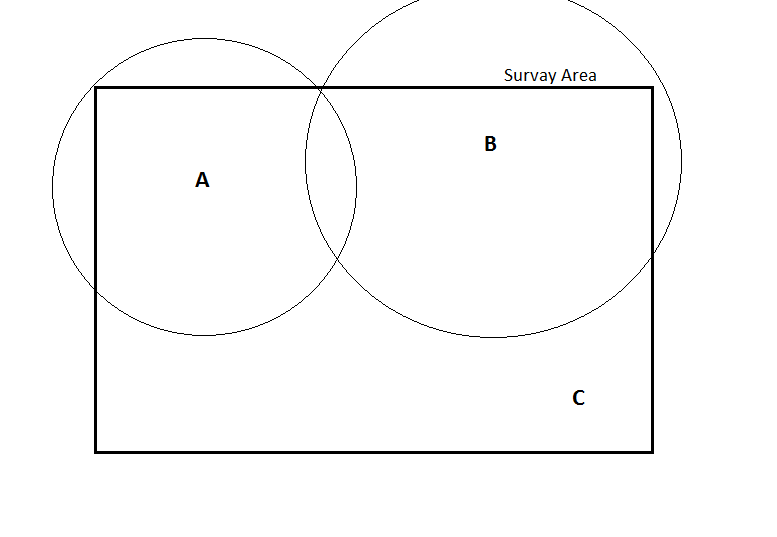
\includegraphics[width=0.8\textwidth]{tri_2.png}
	\caption{Trilateration - Signal Generator B's signal received }
\end{figure*}

This distance is also equally broadcast in all directions. By this time, the receiver has two known distances from two signal generators. The precise position could be at any of the two positions where two circles intersect. With the third signal generator(C), it reveals true location of the receiver where all three circles intersect.

\begin{figure*}[h]	
	\centering
	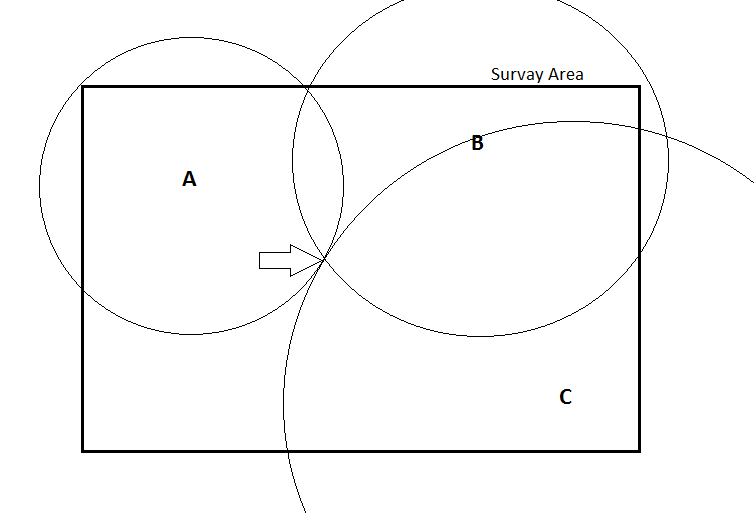
\includegraphics[width=0.8\textwidth]{tri_3.png}
	\caption{Trilateration - Receiver's location }
\end{figure*}

\paragraph{}
There are two types of trilateration techniques available.\cite{trilateration_2}
\begin{enumerate}
	\item 2-D Trilateration
		\subitem In this technique it uses two-dimension(2-D) cartesian plain to locate receiver. The signal generators broadcast their signals in a circular manner. 

	\item 3-D Trilateration
		\subitem In this technique, it uses three-dimension(3-D) cartesian plane to locate receiver. Likewise 2-D trilateration, 3-D trilateration broadcasts its signal in spherical manner.
\end{enumerate}

\paragraph{}
 Trilateration method is being used practically by Global Positioning Service (GPS) satellites to locate users. These satellites broadcast signals in a spherical manner (3-D trilateration) and where all spheres intersect determines the position of the GPS receiver. 
 
 \newpage
 \subsection{HYBRID TECHNIQUE}
 Combination of LOCATION FINGERPRINT TECHNIQUE and TRILATERATION TECHNIQUE is called HYBRID TECHNIQUE.\cite{hybrid_tech} Location fingerprinting technique can fingerprint each location uniquely with respect to Wi-Fi signal strength. By using Trilateration technique, it is possible to locate receiver(user)'s location even inside in a building. With the combination of those two techniques, the receiver's location can be retrieved without using any other locational technique such as GPS. 
 
 \subsection{RADIUS PROTOCOL}
 Remote Authentication Dial-In User Service (RADIUS) is an industrial standard for distributed remote access networking which provides authorization, authentication, accounting and identification.\cite{radius_protocol} Protocol uses Password Authentication Protocol(PAP), Challenge Handshake Protocol(CHAP), Extensible Authentication Protocol(EAP) to authenticate users. RADIUS can look text file,Database or LDAP server for authentication.
 
 \paragraph{}
 The RADIUS server consists of three main authentication responses.
 
 	\begin{itemize}
 		\item Access Accept
 			\subitem Once the user is authenticated, the RADIUS server returns this response. Then the server will often check whether user is authorized or not, to use network. 
 		\item Access Challenge
 			\subitem This requests additional information by server such as PIN, token or secondary password to authenticate the user.
 		\item Access Reject
 			\subitem User is denied to access to all requested network access due to the authentication failure.
 	\end{itemize}
 
 \begin{figure*}[h]	
 	\centering
 	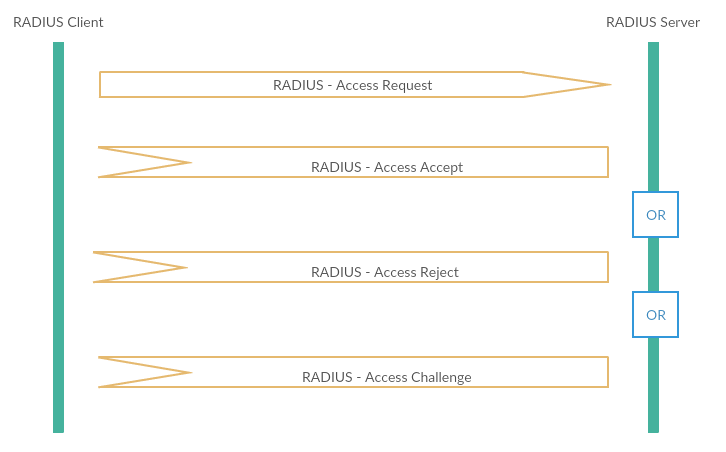
\includegraphics[width=0.8\textwidth]{radius_auth.png}
 	\caption{RADIUS authentication process}
 \end{figure*}
 
 RADIUS client can be any user, who is requesting access from RADIUS server. First user sends Access-Request to the RADIUS server together with user credential information and server checks whether user is valid or not. According to the validation, the server sends appropriate response as per the protocol that server is using for.
 
 \paragraph{}
 For this research project, "FreeRADIUS SERVER" has been used as the RADIUS server.
 
 \paragraph{}
 \begin{center}
 	\begin{table}[H]			
 		\begin{tabu}  { | X[c] | X[c] | }	
 			\hline
 			FreeRADIUS Strengths& FreeRADIUS Weakness \\
 			\hline
 			\begin{itemize}
 				\item Open source
 					\subitem FreeRADIUS is releasd under general public licence. It is free to use, change and whatever fix as required.
 				\item Availability
 					\subitem Supports to all popular Linux distribution and also for Windows operating system.
 				\item Active development
 					\subitem Since FreeRADIUS is an open source and it has world wide development community, FreeRADIUS is being rapidly updated.
 				\item Powerful
 					\subitem FreeRADIUS is capable of supporting file based authentication and  database based authentication.
 				\item Used by mass
 					\subitem Large organizations also use FreeRADIUS not only in sri lanka, but also all around the world.
 			\end{itemize} & 
 			\begin{itemize}
 				\item Complexity
 					\subitem FreeRADIUS offers an all-inclusive piece of software with many configuration options. If any of the configuration is missed or incorrectly configured, it ends up with broken system.
 				\item Vulnerabilities
 					\subitem Few vulnerabilities have been published.
 			\end{itemize}\\
 			\hline
 		\end{tabu}
 		\caption[FreeRADIUS strengths and weaknesses]{FreeRADIUS strengths and weaknesses}
 		\label{table:aimPt_isol}
 	\end{table}
 \end{center} 
 
 
 \subsection{ANDROID WifiEnterpriseConfig API}
 Android WifiEnterpriseConfig application programming interface(API) supports the RADIUS protocol\cite{wpa2_enterprise} from API level 18 and above. For the android mobile application, this API is used to communicate between FreeRADIUS server and user.
 
\section{STEPS FOLLOWED}

\paragraph{}
In this research, HYBRID TECHNIQUE has been used to locate receiver(user)'s location. FreeRADIUS server has been used as authentication server. MySQL is used as relational database. Android WifiEnterpriseConfig API integrated application has been used as Wi-Fi connector. Ubuntu 14.04 server is used as host server. This research process has been done through a series of steps and with phases. The steps that have been carried out throughout the research are as follows.

	\begin{enumerate}
		\item Setup FreeRADIUS server for Wi-Fi user authentication.
		\subitem Reasons for the choice of FreeRADIUS are,
		
		\begin{enumerate}
			\item FreeRADIUS is powerful and allow more customization in configurations.
			\item It is free to use and free to modify.
			\item Capable of supporting PHP server side scripting and MySQL database for the Wi-Fi authentication process.
			\item Supports Ubuntu distribution.					
		\end{enumerate}
			\subitem FreeRADIUS server has been installed to Ubuntu 14.04 virtual host server with PHP and MySQL services. FreeRADIUS server configuration has been modified to execute PHP script and PHP script has been designed to access training database. 
		
		\item Use Wi-Fi enterprise support access point as main Wi-Fi access point. 
			\subitem Normal home use Wi-Fi access points are not supported to RADIUS protocol. in order to support RADIUS protocol, the device should be able to support Wi-Fi enterprise techniques. From the configuration of the access point, it should be possible to configure to redirect the authentication requests from users to the RADIUS server by providing server's IP address and pre-shared secret. When user authentication request is received, the access point does not try to authenticate the user, but the access point redirects the authentication traffic to RADIUS server. The RADIUS server is responsible to authenticate users and provide appropriate response back to the user.
	
		\item Build Android mobile application with WifiEnterpriseConfig API to provide a required data to authenticate Wi-Fi user via FreeRADIUS server. 	
			\subitem This application is supported by providing information for both off-line training phase of location fingerprinting technique and on-line positioning phase. The provided data from the android mobile device to the authentication server would be RSSI values of each Wi-Fi access point, access point specific data, user name, password. All data are in a single Java Script Object Notation(JSON) object and this JSON object is passed to the authentication server via Wi-Fi access point.
		
		\item Fix three(03) Wi-Fi access points together with enterprise support access point to cover entire research area by each, in different locations. 
		\subitem Wi-Fi trilateration technique requires three access points for the location measurement. And with more number of access points, it can take more accurate fingerprint data for a location.
		
		\item Collect selected location data by using developed android mobile application and populate training database with collected location data within RADIUS server.
		\subitem Developed android mobile application consists of training mode. By enabling the training mode, the server can store the Wi-Fi signal data inside the training database. 
		
		\item Analyze collected data from training database and calculate maximum and minimum Wi-Fi RSSI values for each location for each access point and create a new table with extracted data.  
		
		\item Integrate Wi-Fi location fingerprint database with RADIUS server and use the fingerprint database together with user name and password for Wi-Fi user authentication.
		
		\item On-line location analysis process uses training database to authenticate users
		
		\item Analyze results for conclusion.
		
		\item Develop a back end web based application to control Wi-Fi users.
	\end{enumerate}
 
 
 
 

 